% Provenance (never printed): old premiere S material on the oceanic lithosphere
% (ophiolite-type layering, peridotite and gabbro, partial melting by decompression
% at the ridge, hydrothermalism, cooling and subsidence of the lithosphere with
% age); see sources/book2/PROVENANCE.md. Melting from figdata/grade-11/
% ridge_melting.py (adiabat and Hirschmann solidus), depth against age from
% depth_age.py (ETOPO1 and the Seton 2020 age grid). Partial melting is re-founded
% in Year 2 (mantle-melting); fault is Book 1's (g7), normal fault is defined here.
\chapter{Oceanische ruggen en de oceanische lithosfeer}\label{ch:g11:ocean-ridges}

In februari 1977 fotografeerde een cameraslee die 2500 meter diep over de
Galápagosrift in het oosten van de Grote Oceaan werd gesleept, beeld na beeld de
kale zwarte lava van de rug. Toen registreerde de thermometer een kleine stijging
van de watertemperatuur, en op de foto's was de lava bedekt met honderden witte
schelpdieren. Een paar dagen later nam de duikboot \emph{Alvin} twee geologen mee
naar de plek: warm, trillend water stroomde uit spleten in de lava, en eromheen
leefden schelpdieren zo lang als een onderarm, mosselen en witte krabben; bij een
latere duik ook kokerwormen met rode toppen. Niemand had daar leven verwacht, dus
er was geen bioloog aan boord. Dit hoofdstuk legt uit wat de geologen hadden
gevonden: hoe de oceaanbodem bij de ruggen wordt gemaakt, waarom het daar heet is,
en wat ervan wordt terwijl hij zich verwijdert.
% ledger: whoi:alvin-1977

\begin{recall}
Bij de ruggen wordt nieuwe oceaanbodem gemaakt die zich aan beide kanten
verwijdert, zodat zijn ouderdom toeneemt met de afstand tot de as; de ruggen vormen
een stelsel van ongeveer \qty{65000}{km} lang, met een riftdal langs langzame ruggen
en een gladde kam langs snelle (\cref{ch:g11:drift-to-spreading}). Platen bewegen
met een paar centimeter per jaar uit elkaar over een rug, sneller over de
Oost-Pacifische Rug dan over de Midden-Atlantische Rug (\cref{ch:g11:plate-motions}).
De \omterm{def:g11:lithosphere-asthenosphere:lithosphere}{lithosfeer} is de starre buitenste schil, de \omterm{def:g11:lithosphere-asthenosphere:lithosphere}{asthenosfeer} eronder vloeit; de
temperatuur van de \omterm{def:g11:lithosphere-asthenosphere:lithosphere}{asthenosfeer} stijgt maar met ongeveer \qty{0.45}{\celsius} per
kilometer diepte, en de smelttemperatuur van mantelgesteente stijgt met de diepte
(\cref{ch:g11:lithosphere-asthenosphere}). Magma is gesmolten gesteente onder het
oppervlak, basalt het donkere gesteente dat lava vormt wanneer ze afkoelt, en een
breuk een scheur waarlangs gesteenten zijn verschoven (Boek 1, jaar 6 en 7).
\end{recall}
% ledger: noaa:ridge, katsura10:adiabat, hirschmann:solidus

\section{De oceanische lithosfeer}

Twee gesteenten die aan het oppervlak van de continenten zeldzaam zijn, vormen het
grootste deel van de \omterm{def:g11:ocean-ridges:oceanic-lithosphere}{oceanische lithosfeer}.

\begin{definition}[Peridotiet]\label{def:g11:ocean-ridges:peridotite}
\emph{Peridotiet}\index{peridotiet} is een donker, grofkorrelig gesteente dat
vooral bestaat uit het mineraal olivijn, met wat pyroxeen. Het is meestal groen en
dicht. Een groot deel van de aardmantel bestaat vermoedelijk uit peridotiet.
\end{definition}

\begin{definition}[Gabbro]\label{def:g11:ocean-ridges:gabbro}
\emph{Gabbro}\index{gabbro} is een donker, grofkorrelig stollingsgesteente dat
vooral bestaat uit plagioklaas-veldspaat en pyroxeen. Het heeft dezelfde
samenstelling als basalt, maar het kristalliseerde langzaam, diep onder de grond,
waardoor zijn kristallen tijd hadden om te groeien. Het is het meest voorkomende
gesteente van de diepe \omterm{def:g11:ocean-ridges:oceanic-lithosphere}{oceanische korst}.
\end{definition}
% ledger: geo:peridotite, geo:gabbro

De mineralen die hier worden genoemd, olivijn, pyroxeen en veldspaat, worden
beschreven in \cref{ch:g11:minerals}.

\begin{omfigure}
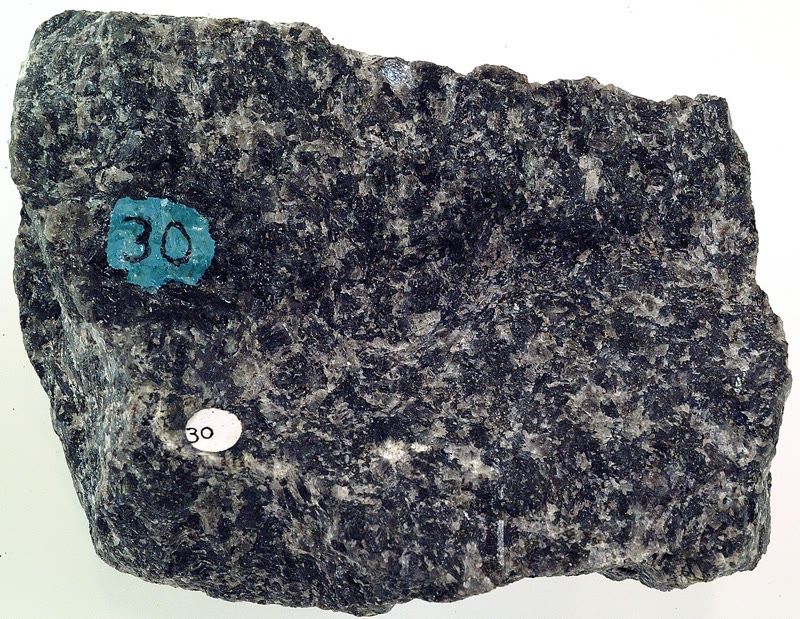
\includegraphics[height=4.2cm]{images/book2/g11-geodil-gabbro.jpg}\hspace{0.03\linewidth}%
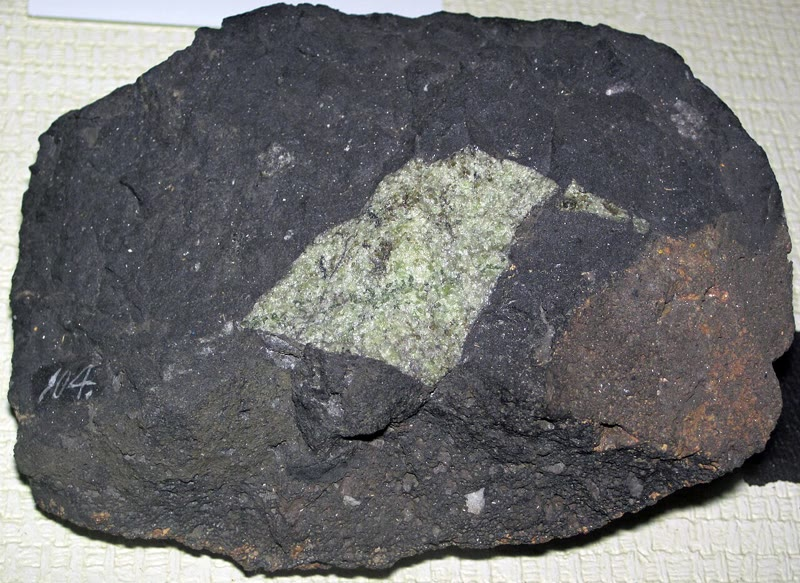
\includegraphics[height=4.2cm]{images/book2/g11-stjohn-peridotite.jpg}

{\small Links: \omterm{def:g11:ocean-ridges:gabbro}{gabbro}, \qty{9}{cm} breed, met donkere pyroxeen- en lichte
veldspaatkristallen die groot genoeg zijn om te zien; foto Darla Sondrol (CC0).
Rechts: een brok groene \omterm{def:g11:ocean-ridges:peridotite}{peridotiet} uit de mantel, meegevoerd in de
zwarte basaltlava van een vulkaan in Arizona; foto James St.~John (CC~BY~2.0).}
\end{omfigure}
% ledger: photo:g11-gabbro, photo:g11-peridotite

\begin{definition}[Oceanische korst; oceanische lithosfeer]\label{def:g11:ocean-ridges:oceanic-lithosphere}
De \emph{oceanische korst}\index{oceanische korst} is de korst van de
oceaanbodem: ongeveer \qty{7}{km} basalt en \omterm{def:g11:ocean-ridges:gabbro}{gabbro}, gemaakt bij de ruggen. De
\emph{oceanische lithosfeer}\index{oceanische lithosfeer} is de oceanische korst
samen met de starre \omterm{def:g11:ocean-ridges:peridotite}{peridotiet} van de bovenste mantel eronder.
\end{definition}

Seismische metingen over alle oceanen geven de \omterm{def:g11:ocean-ridges:oceanic-lithosphere}{oceanische korst} een gemiddelde
dikte van \qty{7.1}{km}, met een marge van \qty{0.8}{km}, buiten breukzones en
hotspots. Haar lagen zijn bekend uit diepe boringen en uit plakken oude oceaanbodem
die op de continenten zijn geschoven. In 2005 voltooide een boorschip een gat van
\qty{1507}{m} diep in 15 miljoen jaar oude korst in het oosten van de Grote
Oceaan, het eerste dat van de lava's, door de gangen, tot in de
\omterm{def:g11:ocean-ridges:gabbro}{gabbro}'s ging:
% ledger: white92:crust, iodp1256:section, geo:peridotite

\begin{itemize}
  \item bovenaan een dun dek van \emph{sedimenten}, afwezig op de as van de
        rug en dikker op oudere bodem;
  \item meer dan \qty{800}{m} \emph{basaltlava's}, op de zeebodem uitgevloeid
        als platen en als \emph{kussens}, ronde buizen en klodders
        lava met een glazige huid;
  \item het \emph{gangencomplex}, \qty{346}{m} in dit gat: honderden
        verticale platen basalt, elk de gestolde spleet waardoor magma
        naar een uitbarsting opsteeg, naast elkaar als de bladzijden van een boek;
  \item \emph{\omterm{def:g11:ocean-ridges:gabbro}{gabbro}}, bereikt op \qty{1407}{m} onder de zeebodem, het magma
        dat onder de gangen langzaam kristalliseerde, tot aan de \omterm{def:g11:seismic-structure:moho}{Moho};
  \item onder de \omterm{def:g11:seismic-structure:moho}{Moho} de \emph{\omterm{def:g11:ocean-ridges:peridotite}{peridotiet}} van de mantel.
\end{itemize}
% ledger: iodp1256:section, geo:basalt-ridges, geo:gabbro

\begin{omfigure}
\begin{tikzpicture}[x=1cm, y=-0.55cm, font=\footnotesize]
% to scale in depth: lavas 0.8 km, dykes 0.35 km (iodp1256:section), crust 7.1 km (white92:crust)
  \fill[omLithAlluv] (0,-0.25) rectangle (2.4,0);
  \fill[lith basalt] (0,0) rectangle (2.4,0.8);
  \fill[omLithBasalt!60] (0,0.8) rectangle (2.4,1.15);
  \foreach \x in {0.15,0.35,...,2.3} \draw[black!55, line width=0.3pt] (\x,0.8) -- (\x,1.15);
  \fill[lith gabbro] (0,1.15) rectangle (2.4,7.1);
  \fill[lith peridotite] (0,7.1) rectangle (2.4,9.0);
  \draw (0,-0.25) rectangle (2.4,9.0);
  \draw[line width=0.9pt] (0,7.1) -- (2.4,7.1);
  \foreach \d in {0,2,4,6,8} {\draw (-0.1,\d) -- (0,\d); \node[anchor=east] at (-0.1,\d) {\d};}
  \node[rotate=90, anchor=south] at (-0.75,4.5) {diepte onder de zeebodem (\unit{km})};
  \draw[black!60] (2.4,-0.13) -- (2.7,-1.0) -- (2.85,-1.0);
  \node[anchor=west] at (2.85,-1.0) {sedimenten};
  \draw[black!60] (2.4,0.4) -- (2.7,0.25) -- (2.85,0.25);
  \node[anchor=west] at (2.85,0.25) {lava's: kussens en plaatvormige stromen};
  \draw[black!60] (2.4,0.98) -- (2.7,1.6) -- (2.85,1.6);
  \node[anchor=west] at (2.85,1.6) {gangencomplex};
  \node[anchor=west] at (2.55,4.1) {gabbro};
  \node[anchor=west] at (2.55,7.1) {Moho};
  \node[anchor=west] at (2.55,8.05) {peridotiet van de mantel};
  \draw[decorate, decoration={brace, amplitude=5pt}] (7.9,0) -- (7.9,7.1)
    node[midway, right=7pt, align=left] {oceanische korst\\ongeveer \qty{7}{km}};
\end{tikzpicture}

{\small De lagen van de \omterm{def:g11:ocean-ridges:oceanic-lithosphere}{oceanische korst}, in de diepte op schaal. De diktes van
de lava's en de gangen zijn die van het diepe gat dat in het oosten van de Grote
Oceaan is geboord; de totale dikte is het gemiddelde uit seismische metingen. Het
sedimentdek wordt dikker met de ouderdom van de bodem.}
\end{omfigure}
% ledger: iodp1256:section, white92:crust

\begin{omfigure}
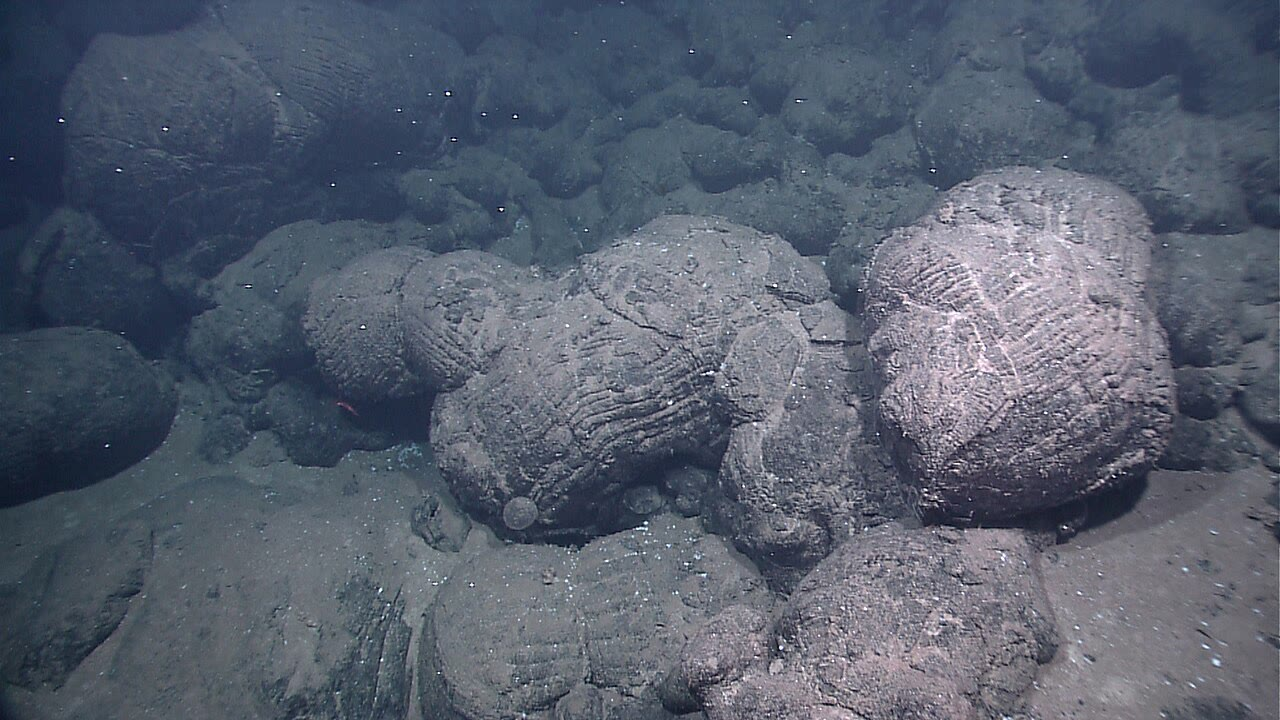
\includegraphics[width=0.8\linewidth]{images/book2/g11-noaa-pillow-lava.jpg}

{\small Kussenlava op de Galápagosrift, ongeveer 2500 meter diep,
gefotografeerd door een op afstand bestuurd voertuig in 2011. Elk kussen is een tong
lava die van buiten stolde op het moment dat ze het koude zeewater raakte.
Foto: NOAA Okeanos Explorer Program (publiek domein).}
\end{omfigure}
% ledger: photo:g11-pillow-lava, whoi:alvin-1977 (depth of the rift floor)

\section{Smelten zonder verhitten}

De mantel onder een rug is vaste \omterm{def:g11:ocean-ridges:peridotite}{peridotiet}, zoals overal elders. Toch komt er
\qty{7}{km} basalt en \omterm{def:g11:ocean-ridges:gabbro}{gabbro} uit, gestold gesmolten gesteente. Waar
komt de smelt vandaan?

\begin{definition}[Partieel smelten; decompressiesmelten]\label{def:g11:ocean-ridges:partial-melting}
\emph{Partieel smelten}\index{partieel smelten} is het smelten van maar een deel
van een gesteente: sommige van zijn mineralen, of sommige van hun bestanddelen,
smelten, terwijl de rest vast blijft.
\emph{Decompressiesmelten}\index{decompressiesmelten} is het partieel smelten van een gesteente dat opstijgt, en dus steeds
minder wordt samengedrukt, zonder te worden verhit.
\end{definition}

Wanneer twee platen uit elkaar bewegen, stijgt de \omterm{def:g11:lithosphere-asthenosphere:lithosphere}{asthenosfeer} onder de rug op om de
ruimte te vullen. Ze stijgt te snel op om veel warmte te verliezen, dus haar
temperatuur daalt onderweg naar boven maar met ongeveer \qty{0.45}{\celsius} per
kilometer. Haar smelttemperatuur, die van de druk afhangt, daalt veel sneller:
ongeveer \qty{3.9}{\celsius} per kilometer op een diepte van \qty{50}{km}. Op een
bepaalde diepte bereikt het opstijgende gesteente zijn smelttemperatuur en begint
het te smelten, hoewel er geen warmte is toegevoegd.
% ledger: katsura10:adiabat, hirschmann:solidus, white92:crust; computed in
% figdata/grade-11/ridge_melting.py (solidus_slope_50km 3.89)

\begin{method}[Waar smelt de opstijgende mantel?]\label{met:g11:ocean-ridges:melting}
\begin{enumerate}
  \item Schrijf de temperatuur van het opstijgende gesteente op elke diepte op: zijn
        potentiële temperatuur (de temperatuur die het aan het oppervlak zou hebben)
        plus \qty{0.45}{\celsius} per kilometer diepte.
  \item Schrijf de smelttemperatuur van het gesteente op elke diepte op, uit de
        druk op die diepte.
  \item Zoek de diepte waarop de twee gelijk zijn. Dieper is het gesteente vast;
        ondieper is het gedeeltelijk gesmolten.
\end{enumerate}
\end{method}

\begin{omfigure}
\begin{tikzpicture}
\begin{axis}[omrecord, omdepth, width=0.72\linewidth, height=6.4cm, xmin=1100, xmax=1700, ymin=0, ymax=150,
  xlabel={temperatuur (\unit{\celsius})}, ylabel={diepte (\unit{km})},
  xticklabel style={/pgf/number format/set thousands separator={}}, clip=true]
% computed in figdata/grade-11/ridge_melting.py; ledger: katsura10:adiabat, hirschmann:solidus, data:prem
\addplot[omProp, line width=1.0pt] table[x=solidus, y=z] {figdata/out/grade-11-ridge_melting-curves.dat};
\addplot[omDef, line width=1.0pt] table[x=ad1300, y=z] {figdata/out/grade-11-ridge_melting-curves.dat};
\addplot[omDef, densely dashed, line width=0.9pt] table[x=ad1400, y=z] {figdata/out/grade-11-ridge_melting-curves.dat};
\addplot[only marks, mark=*, mark size=1.8pt, black] coordinates {(1324.3,54.1) (1438.3,85.0)};
\node[font=\scriptsize, anchor=east, align=right] at (axis cs:1316,62) {smelten begint,\\op \qty{54}{km}};
\node[font=\scriptsize, anchor=east] at (axis cs:1432,89) {\qty{85}{km}};
\node[font=\scriptsize, text=omProp, anchor=west, align=left] at (axis cs:1560,40) {smelt-\\temperatuur};
\node[font=\scriptsize, text=omDef, anchor=east, align=right] at (axis cs:1318,128) {opstijgende mantel,\\$T_p = \qty{1300}{\celsius}$};
\node[font=\scriptsize, text=omDef, anchor=west, align=left] at (axis cs:1476,140) {$T_p = \qty{1400}{\celsius}$};
\end{axis}
\end{tikzpicture}

{\small De temperatuur van mantelgesteente dat onder een rug opstijgt (blauw) en zijn
smelttemperatuur (oranje), tegen de diepte. Gesteente met een potentiële
temperatuur van \qty{1300}{\celsius} begint op \qty{54}{km} diepte te smelten;
gesteente dat \qty{100}{\celsius} heter is (stippellijn) al op \qty{85}{km}.
Smelttemperatuur van droge \omterm{def:g11:ocean-ridges:peridotite}{peridotiet} uit experimenten (Hirschmann, 2000).}
\end{omfigure}
% values: onset_1300_km 54.1, onset_1400_km 85.0, t_onset_1300 1324 (ridge_melting.py)

\begin{example}[De diepte van het smelten]\label{ex:g11:ocean-ridges:onset}
Voor een mantel met potentiële temperatuur \qty{1300}{\celsius} is het opstijgende
gesteente $1300 + 0.45 \times 54 \approx \qty{1324}{\celsius}$ wanneer het
\qty{54}{km} bereikt, precies zijn smelttemperatuur op die diepte: het smelten begint
ongeveer \qty{54}{km} diep. Boven die diepte smelt het verder terwijl het opstijgt.
\end{example}

Maar een klein deel van de \omterm{def:g11:ocean-ridges:peridotite}{peridotiet} smelt, en de smelt is geen \omterm{def:g11:ocean-ridges:peridotite}{peridotiet}:
het is basalt. Basaltsmelten verzamelen zich uit het hele smeltgebied, dat reikt van
de diepte waarop het smelten begint tot aan de onderkant van de korst; omdat ze
lichter zijn dan het vaste gesteente eromheen, stijgen ze op naar de as van de rug.
Daar barst een deel van het magma uit als lava, stolt een deel als gangen in de
spleten waardoor het opsteeg, en kristalliseert een deel langzaam eronder als \omterm{def:g11:ocean-ridges:gabbro}{gabbro}.
De vaste \omterm{def:g11:ocean-ridges:peridotite}{peridotiet} die achterblijft, verarmd aan zijn basalt, wordt het manteldeel
van de \omterm{def:g11:ocean-ridges:oceanic-lithosphere}{oceanische lithosfeer}.
% ledger: asimow01:morb, geo:basalt-ridges, white92:crust

Waar een rug een gebied met hetere mantel kruist, rond een hotspot, begint het
smelten dieper, smelt een langere kolom gesteente en wordt er meer basalt gemaakt:
daar is de korst ongeveer \qty{10}{km} dik in plaats van 7. Omgekeerd heeft de
opstijgende mantel onder heel langzame ruggen tijd om warmte te verliezen, smelt
hij minder, en maakt hij een ongewoon dunne korst.
% ledger: white92:crust

\begin{omfigure}
\begin{tikzpicture}[font=\footnotesize]
  % schematic section across a ridge axis, not to scale
  \fill[omSea!45] (-6,0) rectangle (6,1.2);
  \fill[lith basalt] (-6,0) -- (-0.25,0) -- (-0.25,-0.35) -- (-6,-0.6) -- cycle;
  \fill[lith basalt] (6,0) -- (0.25,0) -- (0.25,-0.35) -- (6,-0.6) -- cycle;
  \fill[lith gabbro] (-6,-0.6) -- (-0.25,-0.35) -- (-0.25,-1.4) -- (-6,-1.6) -- cycle;
  \fill[lith gabbro] (6,-0.6) -- (0.25,-0.35) -- (0.25,-1.4) -- (6,-1.6) -- cycle;
  \fill[lith basalt] (-0.3,0) rectangle (0.3,-0.35);
  \fill[lith gabbro] (-0.3,-0.35) rectangle (0.3,-1.45);
  \fill[omProp!70] (-0.8,-0.75) .. controls (-0.4,-0.55) and (0.4,-0.55) .. (0.8,-0.75)
     .. controls (0.4,-0.95) and (-0.4,-0.95) .. (-0.8,-0.75);
  \fill[omProp!70] (-0.12,0) rectangle (0.12,-0.62);
  \fill[lith peridotite] (-6,-1.6) -- (-0.25,-1.4) -- (0.25,-1.4) -- (6,-1.6) -- (6,-5) -- (-6,-5) -- cycle;
  % melting region
  \fill[omProp!35] (-3.2,-1.5) -- (0,-4.0) -- (3.2,-1.5) -- cycle;
  \node[align=center] at (0,-2.95) {smeltgebied};
  % isotherms deepening away from the axis
  \draw[omDef!70!black, densely dashed] (-6,-2.6) .. controls (-2.5,-2.0) and (-1,-1.1) .. (0,-1.0) .. controls (1,-1.1) and (2.5,-2.0) .. (6,-2.6);
  \draw[omDef!70!black, densely dashed] (-6,-4.2) .. controls (-3,-3.6) and (-1.2,-2.0) .. (0,-1.9) .. controls (1.2,-2.0) and (3,-3.6) .. (6,-4.2);
  \node[text=omDef!70!black, anchor=west] at (6.05,-2.6) {\qty{800}{\celsius}};
  \node[text=omDef!70!black, anchor=west] at (6.05,-4.2) {\qty{1200}{\celsius}};
  % flow arrows
  \draw[-{Stealth[length=5pt]}, line width=0.9pt] (0,-4.9) -- (0,-4.2);
  \draw[-{Stealth[length=5pt]}, line width=0.9pt] (-1.2,-4.8) .. controls (-1.0,-3.8) and (-2.2,-3.2) .. (-3.6,-3.2);
  \draw[-{Stealth[length=5pt]}, line width=0.9pt] (1.2,-4.8) .. controls (1.0,-3.8) and (2.2,-3.2) .. (3.6,-3.2);
  \draw[-{Stealth[length=5pt]}, line width=1.1pt] (-2,0.6) -- (-4,0.6);
  \draw[-{Stealth[length=5pt]}, line width=1.1pt] (2,0.6) -- (4,0.6);
  \node[anchor=south] at (-3,0.65) {plaat};
  \node[anchor=south] at (3,0.65) {plaat};
  \node[anchor=west] at (1.0,-0.8) {magmalens};
  \node[anchor=east] at (-6.05,-0.3) {lava's};
  \node[anchor=east] at (-6.05,-1.1) {gabbro};
  \node[anchor=east] at (-6.05,-3.3) {mantel};
  \node[anchor=north] at (0,-5.05) {de mantel stijgt op en smelt};
\end{tikzpicture}

{\small Een doorsnede over de as van een rug (een tekening, niet op schaal). De
mantel stijgt onder de as op en smelt gedeeltelijk; de smelt verzamelt zich in een
magmalens onder de as en bouwt de korst op, die de platen aan beide kanten
meevoeren. Lijnen van gelijke temperatuur (gestippeld) liggen bij de as dicht bij het
oppervlak en steeds dieper verder ervandaan: de \omterm{def:g11:lithosphere-asthenosphere:lithosphere}{lithosfeer} wordt dikker terwijl ze
afkoelt.}
\end{omfigure}

\section{Snelle en langzame ruggen}

Ruggen gaan met heel verschillende snelheden open. Berekend uit de rotatiepolen van
\cref{ch:g11:plate-motions} gaat de Oost-Pacifische Rug op \ang{30} ZB open met
\qty{14.6}{cm} per jaar, de Midden-Atlantische Rug op dezelfde breedte met
\qty{3.3}{cm} per jaar. De vorm van de as is niet dezelfde.
% ledger: nnr56:poles (computed in plate_velocities.py: epr30s_speed 145.8, atl30s_speed 32.7)

Langs langzame ruggen is de as een dal van 1 tot \qty{2}{km} diep en 20 tot
\qty{30}{km} breed. Er bereikt te weinig magma de as om de ruimte
voortdurend te vullen: de koude, brosse \omterm{def:g11:lithosphere-asthenosphere:lithosphere}{lithosfeer} wordt uit elkaar getrokken en
breekt langs breuken.

\begin{definition}[Afschuiving]\label{def:g11:ocean-ridges:normal-fault}
Een \emph{afschuiving}\index{afschuiving} is een hellende breuk waarlangs het blok
boven het breukvlak naar beneden is bewogen ten opzichte van het blok eronder.
Afschuivingen ontstaan waar de korst wordt uitgerekt.
\end{definition}

Het dal van een langzame rug is een blok dat is weggezakt tussen \omterm{def:g11:ocean-ridges:normal-fault}{afschuivingen} die
naar elkaar toe gekeerd zijn; bijna allemaal hellen ze naar de as. Zo'n weggezakt
blok tussen \omterm{def:g11:ocean-ridges:normal-fault}{afschuivingen} heet een \emph{slenk}.
% ledger: buck05:valley, usgs:normal-fault

Langs snelle ruggen komt er vaak genoeg magma aan om de ruimte te vullen. De as is
een gladde, flauwe verhoging, boven een magmalens die eronder ligt.
% ledger: buck05:valley, noaa:ridge

\begin{omfigure}
\begin{tikzpicture}[font=\footnotesize, x=0.24cm, y=0.9cm]
  % slow ridge: axial valley between normal faults (not to scale, vertical exaggeration)
  \begin{scope}
    \fill[omSea!45] (-15,-0.7) rectangle (15,1.6);
    \fill[lith basalt] (-15,0.9) -- (-9,0.9) -- (-8.5,0.2) -- (-6,0.2) -- (-5.5,-0.6) -- (5.5,-0.6)
      -- (6,0.2) -- (8.5,0.2) -- (9,0.9) -- (15,0.9) -- (15,-2.2) -- (-15,-2.2) -- cycle;
    \draw[black!70] (-15,0.9) -- (-9,0.9) -- (-8.5,0.2) -- (-6,0.2) -- (-5.5,-0.6) -- (5.5,-0.6)
      -- (6,0.2) -- (8.5,0.2) -- (9,0.9) -- (15,0.9);
    \draw[fault] (-9,0.9) -- (-7.4,-2.2);
    \draw[fault] (-6,0.2) -- (-4.6,-2.2);
    \draw[fault] (9,0.9) -- (7.4,-2.2);
    \draw[fault] (6,0.2) -- (4.6,-2.2);
    % slip arrows on the hanging walls (the axis side of each fault): down along the fault
    \foreach \x/\y/\s in {-7.9/-0.5/1, -5.0/-1.3/1, 7.9/-0.5/-1, 5.0/-1.3/-1} {
      \draw[-{Stealth[length=3pt]}, omProp, line width=0.8pt] (\x+0.9*\s,\y+0.45) -- ++(0.3*\s,-0.6);
    }
    \draw[-{Stealth[length=5pt]}, line width=1pt] (-11,1.25) -- (-14,1.25);
    \draw[-{Stealth[length=5pt]}, line width=1pt] (11,1.25) -- (14,1.25);
    \node at (0,-0.25) {axiaal dal};
    \node[anchor=north, align=center] at (0,-2.25) {langzame rug: een dal\\tussen afschuivingen};
  \end{scope}
  % fast ridge
  \begin{scope}[xshift=8.2cm]
    \fill[omSea!45] (-15,0) rectangle (15,1.6);
    \fill[lith basalt] (-15,0.3) .. controls (-6,0.4) and (-2,0.9) .. (0,0.95) .. controls (2,0.9) and (6,0.4) .. (15,0.3)
      -- (15,-2.2) -- (-15,-2.2) -- cycle;
    \fill[omProp!75] (-2.5,-0.9) .. controls (-1,-0.7) and (1,-0.7) .. (2.5,-0.9) .. controls (1,-1.1) and (-1,-1.1) .. (-2.5,-0.9);
    \draw[black!70] (-15,0.3) .. controls (-6,0.4) and (-2,0.9) .. (0,0.95) .. controls (2,0.9) and (6,0.4) .. (15,0.3);
    \node[anchor=north] at (0,-1.25) {magmalens};
    \draw[-{Stealth[length=5pt]}, line width=1pt] (-8,1.25) -- (-14,1.25);
    \draw[-{Stealth[length=5pt]}, line width=1pt] (8,1.25) -- (14,1.25);
    \node at (0,1.3) {axiale verhoging};
    \node[anchor=north, align=center] at (0,-2.25) {snelle rug: een flauwe verhoging\\boven een magmalens};
  \end{scope}
\end{tikzpicture}

{\small Doorsneden over een langzame en een snelle rug (tekeningen, niet op schaal;
de hoogte is overdreven). Links: het axiale dal van een langzame rug, 1 tot
\qty{2}{km} diep, is weggezakt tussen \omterm{def:g11:ocean-ridges:normal-fault}{afschuivingen} die naar de as hellen
(oranje pijlen: de blokken boven de breuken glijden omlaag). Rechts: een snelle rug
rijst flauw op boven een magmalens.}
\end{omfigure}
% ledger: buck05:valley

\begin{example}[Een langzame en een snelle rug]\label{ex:g11:ocean-ridges:rates}
In een miljoen jaar maakt de Oost-Pacifische Rug op \ang{30} ZB
$\qty{14.6}{cm/yr} \times 10^6\ \text{jaar} = \qty{146}{km}$ nieuwe
oceaanbodem, \qty{73}{km} aan elke kant; de Midden-Atlantische Rug op dezelfde breedte
maakt \qty{33}{km}, \qty{16.5}{km} aan elke kant. Het diepe gat in het oosten van de
Grote Oceaan ging in korst die met meer dan \qty{20}{cm} per jaar was gemaakt, een van
de snelste spreidingen die ooit zijn gemeten.
\end{example}
% ledger: nnr56:poles (computed), iodp1256:section

\section{Hydrothermale bronnen}

De jonge korst bij de as is heet, en ze is gebroken door spleten. Zeewater
vindt er zijn weg in.

\begin{definition}[Hydrothermale circulatie; zwarte roker]\label{def:g11:ocean-ridges:hydrothermal}
\emph{Hydrothermale circulatie}\index{hydrothermale circulatie} is de stroming
van zeewater omlaag door de spleten van de hete \omterm{def:g11:ocean-ridges:oceanic-lithosphere}{oceanische korst}, waar het door het
magma eronder wordt verhit en met het gesteente reageert, en terug omhoog naar de
zeebodem, waar het naar buiten komt bij \emph{hydrothermale bronnen}. Een \emph{zwarte
roker}\index{zwarte roker} is een bron waaruit heel heet water met
opgeloste metalen stroomt; wanneer het het koude zeewater raakt, slaan ijzersulfiden en
andere mineralen neer als een zwarte wolk, en bouwen ze een schoorsteen rond de
bron.
\end{definition}
% ledger: whoi:vents

Het water van een \omterm{def:g11:ocean-ridges:hydrothermal}{zwarte roker} verlaat zijn schoorsteen gewoonlijk bij ongeveer
\qty{350}{\celsius}, en bronwater kan \qty{400}{\celsius} bereiken. Het kookt niet,
omdat er tweeënhalve kilometer water op drukt. De
schoorstenen kunnen meer dan \qty{10}{m} hoog worden. Rond de bronnen halen bacteriën
hun energie uit het waterstofsulfide van het bronwater, en voeden ze kokerwormen,
garnalen en mosselen: daarvan leefden de schelpdieren van de Galápagosrift. De meeste
bronnen liggen langs de mid-oceanische ruggen.
% ledger: whoi:vents, whoi:alvin-1977

\begin{omfigure}
\begin{minipage}[c]{0.6\linewidth}\centering
\begin{tikzpicture}[font=\scriptsize, x=0.8cm, y=0.62cm]
  \fill[omSea!45] (0,0) rectangle (10,3);
  \fill[lith basalt] (0,0) rectangle (10,-4);
  \fill[omProp!70] (2,-4.6) .. controls (4,-4.0) and (6,-4.0) .. (8,-4.6) -- (8,-5) -- (2,-5) -- cycle;
  \node at (5,-4.7) {magma};
  \fill[black!75] (4.7,0) -- (4.85,1.6) -- (5.15,1.6) -- (5.3,0) -- cycle;
  \fill[black!45, opacity=0.8] (5,1.7) circle (0.35) (5.2,2.2) circle (0.45) (4.9,2.7) circle (0.4);
  \draw[-{Stealth[length=4pt]}, omDef, line width=0.9pt] (1,0) .. controls (1,-2.5) and (2.5,-3.6) .. (4.2,-3.5);
  \draw[-{Stealth[length=4pt]}, omDef, line width=0.9pt] (9,0) .. controls (9,-2.5) and (7.5,-3.6) .. (5.8,-3.5);
  \draw[-{Stealth[length=4pt]}, omProp, line width=1.1pt] (5,-3.3) -- (5,-0.1);
  \node[align=center, text=omDef!80!black] at (1.6,1.0) {koud zeewater\\stroomt in};
  \node[align=left, anchor=west] at (5.6,1.4) {zwarte roker,\\ongeveer \qty{350}{\celsius}};
  \node[align=left, anchor=west, text=omProp!80!black, fill=white, fill opacity=0.85, text opacity=1, inner sep=1.5pt] at (5.3,-1.8) {verhit,\\stijgt op};
\end{tikzpicture}
\end{minipage}\hfill
\begin{minipage}[c]{0.3\linewidth}\centering
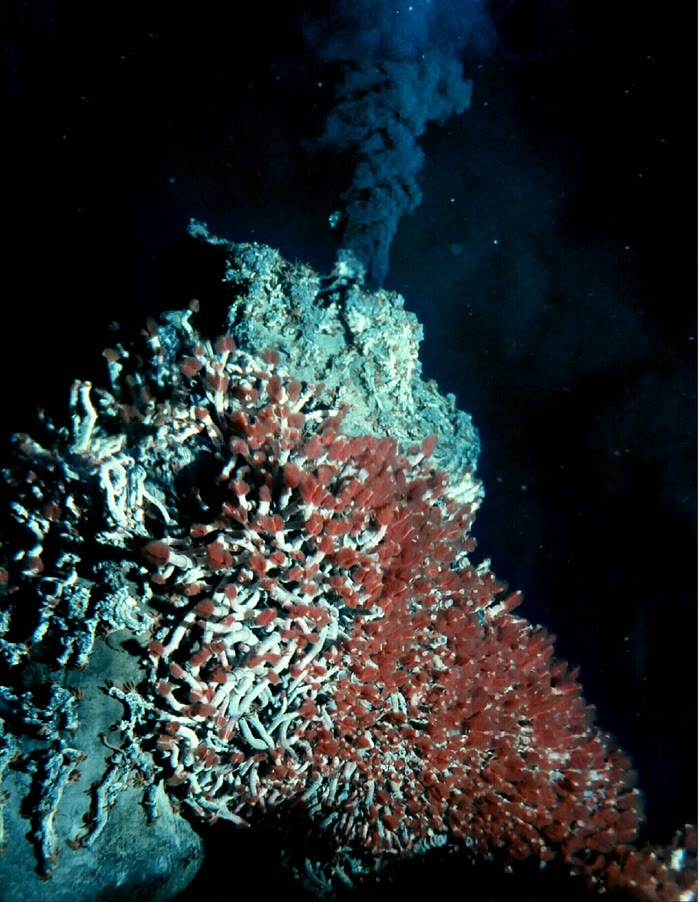
\includegraphics[width=\linewidth]{images/book2/g11-noaa-black-smoker.jpg}
\end{minipage}

{\small Links: \omterm{def:g11:ocean-ridges:hydrothermal}{hydrothermale circulatie} bij de as van een rug (een tekening, niet op
schaal). Rechts: een \omterm{def:g11:ocean-ridges:hydrothermal}{zwarte roker} op de Juan de Fucarug, zijn schoorsteen bedekt
met kokerwormen met rode kieuwen; foto University of Washington en NOAA
(publiek domein).}
\end{omfigure}
% ledger: whoi:vents, photo:g11-black-smoker

\begin{history}[De \emph{Alvin} op de Galápagosrift, 1977]
De expeditie, gefinancierd door de National Science Foundation, begon op
8~februari 1977 aan boord van het onderzoeksschip \emph{Knorr}. De cameraslee ANGUS,
\qty{2500}{m} diep over de rift gesleept, registreerde een stijging van de
watertemperatuur, en op dezelfde beelden toonden zijn foto's honderden witte
schelpdieren en bruine mosselschelpen op de lava. Bij duik 713 van de \emph{Alvin} vonden de
geologen Jack Corliss en Tjeerd van Andel water van \qty{8}{\celsius}
dat trillend uit de spleten kwam, en daarna tot \qty{17}{\celsius}, terwijl het diepe
water eromheen \qty{2}{\celsius} was; witte schelpdieren tot \qty{30}{cm} lang
bedekten een gebied van ongeveer \qty{50}{m} doorsnede. Er was geen bioloog aan boord: de
expeditie was gekomen voor het hete water, en vond een gemeenschap van dieren die
niemand zich had voorgesteld.
\end{history}
% ledger: whoi:alvin-1977

\section{Afkoelen, dikker worden, wegzakken}

Terwijl ze zich van de as verwijdert, koelt de \omterm{def:g11:lithosphere-asthenosphere:lithosphere}{lithosfeer} van boven af, via de
koude oceaan erboven. De afgekoelde laag wordt met de tijd dikker: de
\omterm{def:g11:lithosphere-asthenosphere:lithosphere}{lithosfeer} groeit van een paar kilometer bij de as tot ongeveer honderd
kilometer op oude bodem. Afgekoeld gesteente krimpt en wordt dichter, dus de
\omterm{def:g11:lithosphere-asthenosphere:lithosphere}{lithosfeer} drijft lager op de \omterm{def:g11:lithosphere-asthenosphere:lithosphere}{asthenosfeer} (\omterm{def:g11:lithosphere-asthenosphere:isostasy}{isostasie},
\cref{ch:g11:lithosphere-asthenosphere}): de oceaanbodem zakt weg naarmate hij ouder wordt.
Voor een lichaam dat door geleiding vanaf zijn oppervlak afkoelt, groeit de dikte van de
afgekoelde laag als de vierkantswortel van de tijd.
% ledger: ps77:depth-age, rs09:lab

\begin{proposition}[Diepte van de oceaanbodem tegen zijn ouderdom]\label{prop:g11:ocean-ridges:depth-age}
Gemiddeld ligt oceaanbodem met ouderdom $t$ (in miljoen jaar) op de diepte
\[
  d(t) = 2500 + 350\sqrt{t} \quad \text{meter} \qquad (0 \le t \le 70),
\]
en, voor bodem die ouder is dan ongeveer 20 miljoen jaar,
\[
  d(t) = 6400 - 3200\,e^{-t/62.8} \quad \text{meter}:
\]
de bodem zakt snel weg zolang hij jong is, en dan steeds langzamer, naar
ongeveer \qty{6400}{m}. (Aangenomen: de formules zijn aangepast aan de diepten van
het noorden van de Grote en de Atlantische Oceaan, gecorrigeerd voor het gewicht van
hun sedimenten, door Parsons en Sclater in 1977.)
\end{proposition}
% ledger: ps77:depth-age

De vierkantswortel laat de jonge bodem snel wegzakken: in zijn eerste miljoen jaar
zakt de bodem \qty{350}{m}, in de volgende drie miljoen jaar nog eens
\qty{350}{m}, en tussen 16 en 64 miljoen jaar \qty{1400}{m}, evenveel als
in zijn eerste zestien miljoen jaar. De exponentiële wet beschrijft hoe oude
bodem ophoudt met wegzakken: hij gedraagt zich alsof de afkoelende plaat een vaste
dikte had, ongeveer \qty{125}{km}.
% ledger: ps77:depth-age

\begin{omfigure}
\begin{tikzpicture}
\begin{axis}[omrecord, omdepth, width=0.82\linewidth, height=6.2cm, xmin=0, xmax=180, ymin=2000, ymax=6600,
  xlabel={ouderdom van de oceaanbodem (miljoen jaar)}, ylabel={diepte (\unit{m})},
  yticklabel style={/pgf/number format/set thousands separator={}},
  legend style={font=\scriptsize, at={(0.5,-0.32)}, anchor=north, legend columns=3, /tikz/every even column/.append style={column sep=6pt}}, legend cell align=left]
% computed in figdata/grade-11/depth_age.py; ledger: data:etopo1, data:b2-seafloor-age, ps77:depth-age
\addplot[only marks, mark=*, mark size=1.3pt, black!70, error bars/.cd, y dir=both, y explicit]
  table[x=age, y=depth, y error minus=em, y error plus=ep] {figdata/out/grade-11-depth_age-bins.dat};
\addplot[omProp, line width=1.0pt] table[x=age, y=depth] {figdata/out/grade-11-depth_age-sqrt.dat};
\addplot[omDef, line width=1.0pt, densely dashed] table[x=age, y=depth] {figdata/out/grade-11-depth_age-exp.dat};
\legend{{gemeten: mediaan en middelste helft}, {$2500 + 350\sqrt{t}$}, {$6400 - 3200\,e^{-t/62.8}$}}
\end{axis}
\end{tikzpicture}

{\small Diepte van de oceaanbodem tegen zijn ouderdom: voor elke ouderdomsband van
5 miljoen jaar de mediane diepte van alle cellen van één graad van de oceanen van de
wereld, en het bereik van de middelste helft ervan. Jonge bodem volgt de
wortelwet nauwkeurig; oudere bodem ligt ondieper dan de wetten, omdat
zijn cellen sedimenten en vulkanen bevatten. Gegevens: ETOPO1 (NOAA) en de
ouderdommen van de oceaanbodem van Seton en anderen (2020); wetten van Parsons en Sclater
(1977).}
\end{omfigure}
% values (depth_age.py): median 2.5-5 Myr 3114 (law 3178), 60-65 Myr 4648 (law 5267), fit a 2727 b 255

De gemeten diepten van jonge bodem komen tot op ongeveer \qty{100}{m} overeen met
de wet. Op oudere bodem liggen de gemeten medianen een paar honderd meter
boven de wetten. De wetten beschrijven de diepte van de bodem zelf, alsof zijn
sedimenten waren verwijderd; de gemeten cellen dragen hun sedimenten nog,
die dikker worden met de ouderdom van de bodem en meer dan een kilometer
dik zijn op de oudste bodem van het westen van de Noord-Atlantische Oceaan, en ze
bevatten onderzeese bergen en vulkanische plateaus.
% ledger: ps77:depth-age; values from depth_age.py

Oude \omterm{def:g11:ocean-ridges:oceanic-lithosphere}{oceanische lithosfeer} is dus dik, koud en dicht. Het volgende hoofdstuk
laat zien dat ze dichter kan worden dan de \omterm{def:g11:lithosphere-asthenosphere:lithosphere}{asthenosfeer} eronder, en terug kan
zakken in de mantel (\cref{ch:g11:subduction-zones}).

\section{Oefeningen}

\begin{exercise}[$\star$]\label{exo:g11:ocean-ridges:1}
Definieer \omterm{def:g11:ocean-ridges:peridotite}{peridotiet} en \omterm{def:g11:ocean-ridges:gabbro}{gabbro}. Welke van de twee hoort bij de \omterm{def:g11:ocean-ridges:oceanic-lithosphere}{oceanische korst},
en welke bij de mantel? \omterm{def:g11:ocean-ridges:gabbro}{Gabbro} heeft dezelfde samenstelling als basalt: waarom zijn
zijn kristallen zoveel groter?
\end{exercise}

\begin{exercise}[$\star$]\label{exo:g11:ocean-ridges:2}
Noem de lagen van de \omterm{def:g11:ocean-ridges:oceanic-lithosphere}{oceanische lithosfeer} van de zeebodem naar beneden. Het diepe
gat in het oosten van de Grote Oceaan bereikte \qty{1507}{m} onder de zeebodem: welk
deel van een korst van \qty{7.1}{km} heeft het doorkruist?
\end{exercise}

\begin{exercise}[$\star$]\label{exo:g11:ocean-ridges:3}
Bereken met $d = 2500 + 350\sqrt{t}$ de diepte van oceaanbodem van 0, 9 en 25
miljoen jaar oud.
\end{exercise}

\begin{exercise}[$\star$]\label{exo:g11:ocean-ridges:4}
Definieer een \omterm{def:g11:ocean-ridges:normal-fault}{afschuiving}. Welke kracht maakt bij een langzame rug \omterm{def:g11:ocean-ridges:normal-fault}{afschuivingen}, en
in welke richting bewegen de blokken boven de breuken?
\end{exercise}

\begin{exercise}[$\star$]\label{exo:g11:ocean-ridges:5}
Het water van een \omterm{def:g11:ocean-ridges:hydrothermal}{zwarte roker} komt naar buiten bij ongeveer \qty{350}{\celsius}. Waarom
kookt het niet? Wat is de zwarte ``rook''?
\end{exercise}

\begin{exercise}[$\star\star$]\label{exo:g11:ocean-ridges:6}
Gebruik de smeltfiguur: (1) op welke diepte begint een mantel met potentiële
temperatuur \qty{1300}{\celsius} te smelten, en bij welke temperatuur? (2)
En een mantel die \qty{100}{\celsius} heter is? (3) Welke van de twee maakt de
dikkere korst? Waarom?
\end{exercise}

\begin{exercise}[$\star\star$]\label{exo:g11:ocean-ridges:7}
Opstijgend mantelgesteente met potentiële temperatuur \qty{1300}{\celsius} is
\qty{1345}{\celsius} op een diepte van \qty{100}{km}, waar zijn smelttemperatuur
\qty{1489}{\celsius} is. (1) Hoeveel ligt het onder zijn
smelttemperatuur? (2) Het begint te smelten op \qty{54}{km}. Met hoeveel graden
per kilometer is het verschil onderweg naar boven gemiddeld gekrompen? (3) Is het
gesteente verhit?
\end{exercise}

\begin{exercise}[$\star\star$]\label{exo:g11:ocean-ridges:8}
De Oost-Pacifische Rug gaat op \ang{30} ZB open met \qty{14.6}{cm} per jaar, de
Midden-Atlantische Rug met \qty{3.3}{cm} per jaar. Hoe lang heeft elke rug, bij
symmetrische spreiding, nodig om aan één kant \qty{1000}{km} bodem te maken?
\end{exercise}

\begin{exercise}[$\star\star$]\label{exo:g11:ocean-ridges:9}
De ruggen zijn ongeveer \qty{65000}{km} lang. Stel dat ze gemiddeld opengaan met
\qty{5}{cm} per jaar en een korst van \qty{7.1}{km} dik maken. (1) Welke oppervlakte
nieuwe oceaanbodem maken ze per jaar? (2) Welk volume korst? (3) Hoe lang
zouden ze nodig hebben om een oppervlakte te maken die gelijk is aan die van de oceanen,
\qty{3.6e8}{km^2}?
\end{exercise}

\begin{exercise}[$\star\star$]\label{exo:g11:ocean-ridges:10}
Een axiaal dal is \qty{1.5}{km} diep. Het is weggezakt langs twee \omterm{def:g11:ocean-ridges:normal-fault}{afschuivingen}
die naar elkaar toe gekeerd zijn en elk onder \ang{60} hellen. (1) Hoeveel is elke breuk
langs haar vlak verschoven? (2) Hoe ver zijn de twee kanten horizontaal uit elkaar
bewogen door de twee breuken? (3) Het dal is \qty{25}{km} breed: heeft breukvorming
alleen het gemaakt?
\end{exercise}

\begin{exercise}[$\star\star$]\label{exo:g11:ocean-ridges:11}
Bereken met $d = 6400 - 3200\,e^{-t/62.8}$ de diepte van bodem van 25 en 100
miljoen jaar oud, en hoeveel de bodem tussen deze ouderdommen wegzakt. Vergelijk
de eerste waarde met die van de wortelwet.
\end{exercise}

\begin{exercise}[$\star\star\star$]\label{exo:g11:ocean-ridges:12}
Een kolom mantel van \qty{100}{km} dik koelt gemiddeld \qty{700}{\celsius} af.
Gesteente krimpt met $\alpha = 3.2 \times 10^{-5}$ van zijn lengte per
graad afkoeling. (1) Hoeveel wordt de kolom korter? (2) Terwijl ze
wegzakt, vult zeewater (\qty{1025}{kg/m^3}) de ruimte erboven; met een
manteldichtheid van \qty{3380}{kg/m^3} laat \omterm{def:g11:lithosphere-asthenosphere:isostasy}{isostasie} de bodem wegzakken met
$s = \rho_m\,\alpha\,\Delta T\,L/(\rho_m - \rho_w)$. Bereken $s$. (3) Vergelijk
met het totale wegzakken dat de exponentiële wet toelaat, van \qty{2500}{m} tot
\qty{6400}{m}.
\end{exercise}

\begin{exercise}[$\star\star\star$]\label{exo:g11:ocean-ridges:13}
Het smelten begint op \qty{54}{km} diepte in een mantel van \qty{1300}{\celsius},
op \qty{85}{km} diepte in een mantel van \qty{1400}{\celsius}; in beide gaat het
smelten door tot de onderkant van de korst, ongeveer \qty{7}{km} diep. (1) Vergelijk
de lengtes van de twee smeltkolommen. (2) Als elke kilometer opstijgend gesteente
evenveel smelt gaf, hoe dik zou de korst dan zijn boven de hetere mantel, bij een
korst van \qty{7.1}{km} boven de normale? (3) Vergelijk met de \qty{10.3}{km}
die is gemeten waar ruggen hetere mantel ontmoeten.
\end{exercise}

\begin{exercise}[$\star\star\star$]\label{exo:g11:ocean-ridges:14}
De gemeten mediane diepten van de oceaanbodem zijn \qty{3114}{m} bij een ouderdom van
\num{3.75} miljoen jaar, \qty{4018}{m} bij \num{22.5}, \qty{4465}{m} bij
\num{42.5} en \qty{4648}{m} bij \num{62.5}. (1) Bereken de diepte die de
wortelwet bij elke ouderdom geeft, en het verschil met de meting. (2)
Hoe verandert het verschil met de ouderdom? (3) Verklaar het.
\end{exercise}

\begin{exercise}[$\star\star\star$]\label{exo:g11:ocean-ridges:15}
Het kritieke punt van water ligt bij \qty{374}{\celsius} en \qty{22.064}{MPa}: boven
die druk kookt water bij geen enkele temperatuur. (1) Bereken de
druk van het water op \qty{2500}{m} diepte (zeewater \qty{1025}{kg/m^3},
$g = \qty{9.8}{m/s^2}$, plus de \qty{0.1}{MPa} van de atmosfeer). (2) Kan het
water van een bron op die diepte koken, hoe heet het ook is? (3) Onder ongeveer welke
diepte geldt dit voor elke bron?
\end{exercise}

\section{Probleem: het leven van een stuk Pacifische bodem}

\begin{problem}[{Weekendprobleem --- van de rug naar de diepe oceaan}]
\label{pb:g11:ocean-ridges:1}
% values: EPR 30 S full rate 145.8 mm/yr (plate_velocities.py, nnr56:poles); depth law
% ps77:depth-age; crust white92:crust; alpha ps77; densities data:prem; median 60-65 Myr
% 4648 m (depth_age.py)
Een stuk oceaanbodem wordt vandaag geboren op de Oost-Pacifische Rug op \ang{30}
ZB, waar de Pacifische en de Nazcaplaat met \qty{14.6}{cm} per jaar uit elkaar bewegen.
Het beweegt met de Pacifische plaat naar het westen. Neem de spreiding symmetrisch, de
korst \qty{7.1}{km} dik, en de dieptewet $d = 2500 + 350\sqrt{t}$ meter
($t$ in miljoen jaar).

\medskip
\noindent\textbf{Deel I --- Geboorte bij de rug.}
\begin{enumerate}
  \item Wat is de halve \omterm{def:g11:drift-to-spreading:spreading-rate}{spreidingssnelheid}, in centimeter per jaar en in
        kilometer per miljoen jaar?
  \item Op welke diepte wordt het stuk bodem geboren?
  \item Noem de gesteenten waaruit het bestaat, van de zeebodem tot de onderkant van
        de \omterm{def:g11:lithosphere-asthenosphere:lithosphere}{lithosfeer}.
  \item Het magma dat het maakte, kwam uit de mantel eronder. Leg uit hoe de
        mantel smolt zonder te worden verhit.
  \item Welk volume korst maakt deze rug per miljoen jaar, aan
        beide kanten, per kilometer van zijn lengte?
\end{enumerate}

\medskip
\noindent\textbf{Deel II --- De reis.}
\begin{enumerate}[resume]
  \item Hoe ver van de rug zal het stuk na 1, 4, 16 en 64
        miljoen jaar zijn, als de snelheid gelijk blijft?
  \item Hoe lang zal het erover doen om \qty{2000}{km} af te leggen?
  \item Waarom kan de echte afstand na 64 miljoen jaar verschillen van het
        antwoord op vraag~6?
  \item Dicht bij de rug circuleert zeewater door de jonge korst en
        komt het naar buiten bij bronnen. Waarom stopt deze circulatie op oude bodem?
  \item Op welke plaat reist het stuk, en naar welk soort
        plaatgrens voert die plaat het, aan haar westkant?
\end{enumerate}

\medskip
\noindent\textbf{Deel III --- Wegzakken naarmate het ouder wordt.}
\begin{enumerate}[resume]
  \item Bereken zijn diepte bij 1, 4, 16 en 64 miljoen jaar.
  \item Hoeveel zakt het weg in zijn eerste 16 miljoen jaar, en
        tussen 16 en 64 miljoen jaar? Geef commentaar.
  \item Bij welke ouderdom bereikt het een diepte van \qty{4000}{m}?
  \item Vergelijk zijn diepte bij 64 miljoen jaar met de exponentiële wet,
        $6400 - 3200\,e^{-t/62.8}$.
  \item De gemeten mediane diepte van oceaanbodem van 60 tot 65 miljoen jaar oud
        is \qty{4648}{m}. Verklaar het verschil.
\end{enumerate}

\medskip
\noindent\textbf{Deel IV --- Zijn dichtheid en zijn lot.}
\begin{enumerate}[resume]
  \item Neem bij 64 miljoen jaar zijn \omterm{def:g11:lithosphere-asthenosphere:lithosphere}{lithosfeer} \qty{100}{km} dik en
        gemiddeld \qty{700}{\celsius} kouder dan de \omterm{def:g11:lithosphere-asthenosphere:lithosphere}{asthenosfeer}. Met
        $\alpha = 3.2 \times 10^{-5}$ per graad, met welk deel is het
        manteldeel dan dichter geworden? Uitgaande van \qty{3380}{kg/m^3}, wat is
        zijn dichtheid?
  \item Zijn korst is \qty{7.1}{km} dik, met een dichtheid van
        \qty{2900}{kg/m^3}. Bereken de gemiddelde dichtheid van de hele
        \qty{100}{km} \omterm{def:g11:lithosphere-asthenosphere:lithosphere}{lithosfeer}.
  \item Vergelijk met de \omterm{def:g11:lithosphere-asthenosphere:lithosphere}{asthenosfeer} eronder, genomen als
        \qty{3380}{kg/m^3}.
  \item Wat kan zo'n \omterm{def:g11:lithosphere-asthenosphere:lithosphere}{lithosfeer} doen wanneer ze een trog bereikt?
  \item Besluit: op welke diepte ligt dit stuk bodem wanneer het 64
        miljoen jaar oud is?
\end{enumerate}
\end{problem}
